\chapter*{chapitre 5}
\markboth{Chapitre 5 }{5 Release 2 : Services avancés} %pour afficher l'entete
 \addcontentsline{toc}{chapter}{5 Release 2 : Services avancés}

\textbf{\Huge Release 2 : Services avancés}

\setcounter{chapter}{5}
\setcounter{section}{0}

\section{Introduction}

La Release 1 a livré le cas d'utilisation central de la plateforme — le déploiement sécurisé d'une application — ainsi que les briques techniques de Knative Eventing, exploitées jusqu'ici uniquement au niveau du backend. La Release 2 a pour objectif d'exposer ces briques comme de véritables services applicatifs accessibles aux clients (gestion de Kafka et de l'Eventing au travers de l'API), et de doter la plateforme des capacités de supervision nécessaires à son exploitation en conditions réelles : métriques, journaux et détection automatique d'anomalies. Elle regroupe le Sprint 6 et le Sprint 7.


\section{Sprint 6 : Gestion Kafka et Eventing côté Backend}

\subsection{Introduction}

Ce sprint a pour objectif de transformer les capacités techniques de gestion de Kafka (Sprint 2) et de Knative Eventing (Sprint 3), jusque-là exploitées uniquement en interne par le backend, en véritables services applicatifs exposés aux clients au travers de l'API REST, avec les contrôles d'appartenance et de permission requis par le modèle multi-tenant.

\subsection{Objectifs du Sprint}

\begin{itemize}
    \item Exposer, au travers de l'API REST, les opérations de création, de consultation et de suppression des sujets Kafka d'un client.
    \item Exposer, au travers de l'API REST, les opérations de configuration des déclencheurs d'événement (association d'un sujet Kafka à une application).
    \item Garantir que ces opérations respectent strictement l'isolation multi-tenant, y compris pour les utilisateurs de type MEMBER.
\end{itemize}

\subsection{Sprint Backlog}

\begin{table}[!ht]
\begin{center}
     \begin{tabular}{|l{11cm}|l{3cm}|}
     \hline
     \textbf{User Story} & \textbf{Statut} \\
     \hline
     En tant que client, je veux créer un sujet Kafka pour mon compte & Réalisé \\
     \hline
     En tant que client, je veux lister et supprimer mes sujets Kafka & Réalisé \\
     \hline
     En tant que client, je veux configurer un déclencheur reliant un sujet à une application & Réalisé \\
     \hline
     En tant que MEMBER, je veux que mes actions Kafka/Eventing soient rattachées au bon compte client & Réalisé (après correction) \\
     \hline
     \end{tabular}
     \caption{Sprint Backlog — Sprint 6}
     \label{tab:sb-sprint6}
     \end{center}
\end{table}

\subsection{Diagramme de cas d'utilisation du Sprint}

\begin{figure}[h!]
 \centering
    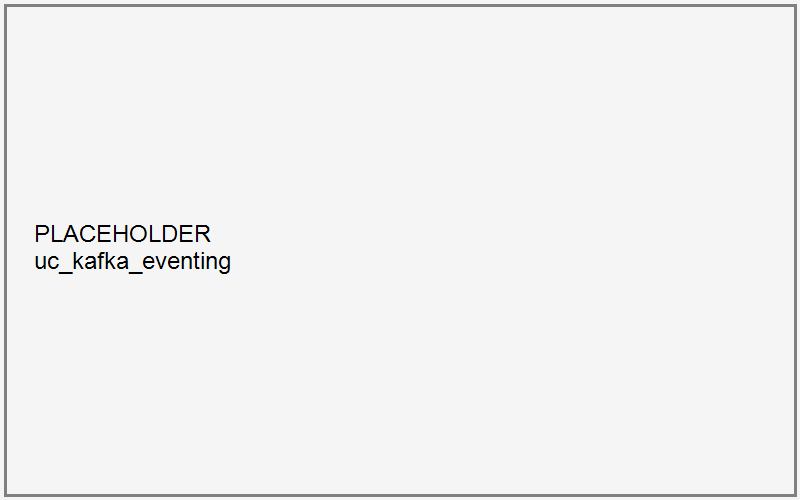
\includegraphics[width=12cm]{diagrammes/uc_kafka_eventing.png}
    \caption{Diagramme de cas d'utilisation — Gestion Kafka et Eventing}
    \label{fig:uc-kafka}
\end{figure}

\subsection{Présentation des composants développés}

\begin{itemize}
    \item \texttt{KafkaController} : expose les points d'accès REST de création, de listing et de suppression des sujets Kafka d'un tenant, en s'appuyant sur \texttt{KafkaService} (Sprint 2) pour l'interaction avec la ressource \texttt{KafkaTopic}.
    \item \texttt{EventingController} : expose les points d'accès REST de configuration des déclencheurs (\texttt{Trigger}/\texttt{KafkaSource}), en s'appuyant sur \texttt{EventingService} (Sprint 3).
    \item Intégration systématique de \texttt{UserContextService} dans ces deux contrôleurs, afin de garantir que toute opération est rattachée à l'identité effective de l'appelant (compte CLIENT\_ADMIN, y compris lorsque l'appelant est un MEMBER).
\end{itemize}

\subsection{Description du cas d'utilisation « Créer un sujet Kafka »}

\subsubsection{Description textuelle}

\begin{table}[!ht]
\begin{center}
     \begin{tabular}{|l{3.5cm}|p{9cm}|}
     \hline
     \textbf{Nom} & Créer un sujet Kafka \\
     \hline
     \textbf{Acteur} & CLIENT\_ADMIN, MEMBER (avec permission de gestion Kafka) \\
     \hline
     \textbf{Pré-condition} & L'utilisateur est authentifié et dispose de la permission requise \\
     \hline
     \textbf{Scénario nominal} & 1. L'utilisateur soumet un nom de sujet. 2. Le backend résout l'identité effective (compte propriétaire) de l'appelant. 3. Le backend crée la ressource \texttt{KafkaTopic} rattachée au cluster Kafka du tenant. 4. Le sujet créé est renvoyé à l'utilisateur et devient disponible pour la configuration de déclencheurs. \\
     \hline
     \textbf{Post-condition} & Le sujet est disponible pour publication/consommation et pour association à une application via un Trigger. \\
     \hline
     \end{tabular}
     \caption{Description textuelle du cas d'utilisation « Créer un sujet Kafka »}
     \label{tab:uc-create-topic}
     \end{center}
\end{table}

\subsubsection{Diagramme de séquence}

\begin{figure}[h!]
 \centering
    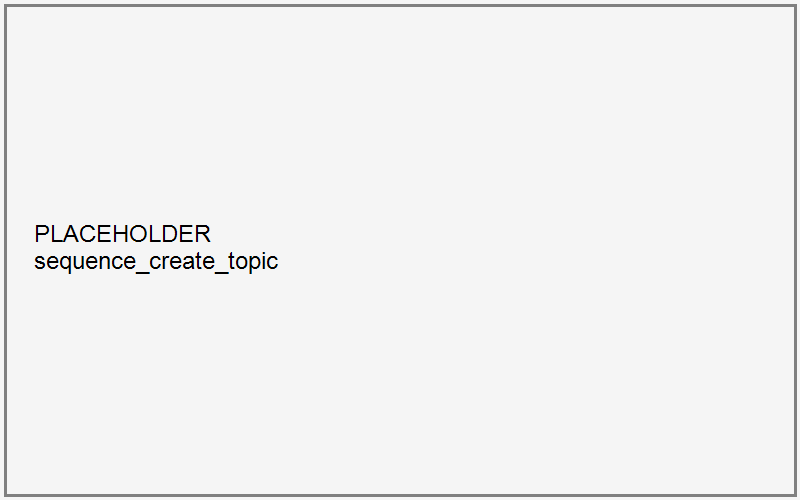
\includegraphics[width=14cm]{diagrammes/sequence_create_topic.png}
    \caption{Diagramme de séquence — Création d'un sujet Kafka}
    \label{fig:seq-create-topic}
\end{figure}

\subsection{Difficultés rencontrées et solutions apportées}

\begin{itemize}
    \item \textbf{Isolation multi-tenant rompue pour les membres d'équipe} : les contrôleurs Kafka et Eventing utilisaient initialement directement l'identifiant d'authentification brut (\texttt{auth.getName()}) au lieu de l'identifiant effectif résolu par \texttt{UserContextService}. Un utilisateur MEMBER pouvait ainsi voir ses ressources Kafka/Eventing rattachées à son propre identifiant plutôt qu'à celui de son compte CLIENT\_ADMIN, cassant le modèle de délégation de propriété établi au Sprint 4 et pouvant conduire à des incohérences d'accès entre membres d'une même équipe. \textit{Solution} : remplacement systématique de ces appels par la résolution via \texttt{UserContextService}, alignant ce module sur le reste du backend.
\end{itemize}

\subsection{Résultat obtenu}

À l'issue de ce sprint, un client peut créer, consulter et supprimer ses sujets Kafka, et configurer des déclencheurs d'événement reliant ses sujets à ses applications, directement au travers de l'API REST, avec une isolation multi-tenant correctement appliquée y compris pour les membres d'équipe. L'exposition de ces fonctionnalités dans l'interface graphique du portail interviendra au Sprint 8.

\subsection{Conclusion du Sprint}

Ce sprint a complété le triptyque applicatif Serverless/Kafka/Eventing initié dès la Release 0, en le rendant pleinement exploitable par les clients au travers de l'API. Le sprint suivant s'attache désormais à doter la plateforme de capacités de supervision, indispensables à son exploitation.


\section{Sprint 7 : Monitoring, métriques et gestion des logs}

\subsection{Introduction}

Ce sprint a pour objectif de doter la plateforme des capacités d'observabilité nécessaires à son exploitation : consultation des journaux applicatifs et de déploiement par les clients, supervision de l'état du cluster par l'équipe d'exploitation, et détection automatique des applications en échec récurrent.

\subsection{Objectifs du Sprint}

\begin{itemize}
    \item Exposer aux clients les journaux de déploiement et les journaux applicatifs (logs des conteneurs) de leurs applications, en temps réel.
    \item Intégrer Prometheus pour la collecte des métriques du backend et des révisions Knative.
    \item Exposer à l'équipe d'exploitation une vue de supervision du cluster (nœuds, alertes actives, usage par tenant) au travers de la console d'administration.
    \item Mettre en place une détection automatique des redémarrages en boucle (\textit{crash loops}) des applications clientes.
\end{itemize}

\subsection{Sprint Backlog}

\begin{table}[!ht]
\begin{center}
     \begin{tabular}{|l{11cm}|l{3cm}|}
     \hline
     \textbf{User Story} & \textbf{Statut} \\
     \hline
     En tant que client, je veux consulter en temps réel les journaux de mon application & Réalisé \\
     \hline
     En tant qu'exploitant, je veux que les métriques du backend soient collectées par Prometheus & Réalisé (avec anomalie identifiée) \\
     \hline
     En tant qu'exploitant, je veux visualiser l'état des nœuds et les alertes actives du cluster & Réalisé \\
     \hline
     En tant qu'exploitant, je veux être informé automatiquement d'une application en boucle de redémarrage & Réalisé \\
     \hline
     \end{tabular}
     \caption{Sprint Backlog — Sprint 7}
     \label{tab:sb-sprint7}
     \end{center}
\end{table}

\subsection{Diagramme de cas d'utilisation du Sprint}

\begin{figure}[h!]
 \centering
    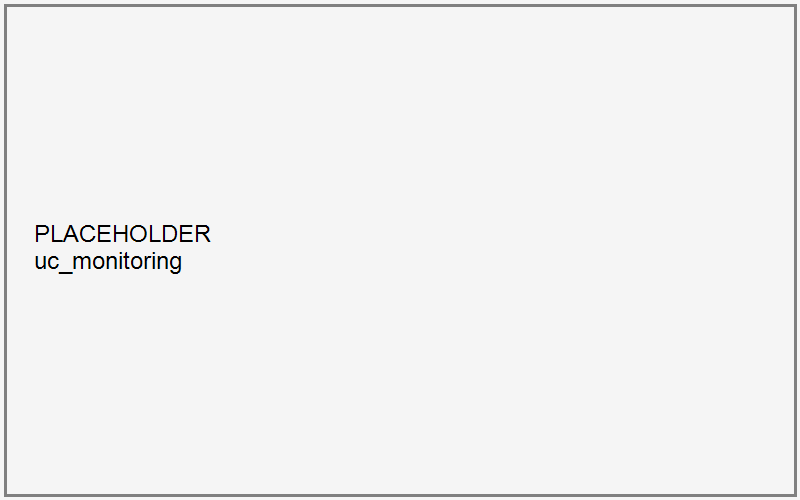
\includegraphics[width=12cm]{diagrammes/uc_monitoring.png}
    \caption{Diagramme de cas d'utilisation — Monitoring et logs}
    \label{fig:uc-monitoring}
\end{figure}

\subsection{Présentation des composants développés}

\begin{itemize}
    \item \texttt{PodLogService} / \texttt{PodLogStreamService} : récupération et diffusion en flux continu des journaux d'un pod applicatif via l'API Kubernetes.
    \item \texttt{LogSseService} : hub de diffusion en temps réel (Server-Sent Events) des journaux de déploiement et applicatifs vers le portail client.
    \item \textbf{Prometheus / Micrometer} : exposition des métriques du backend via le point d'accès \texttt{/actuator/prometheus}, collecte configurée par une ressource \texttt{ServiceMonitor} ; collecte des métriques par révision Knative (latence, concurrence) via une ressource \texttt{PodMonitor} ciblant le conteneur \textit{queue-proxy} de chaque révision.
    \item \texttt{AlertmanagerService} : interrogation de l'API d'Alertmanager pour remonter les alertes actives dans la console d'administration.
    \item \texttt{CrashLoopScheduler} : tâche planifiée interrogeant périodiquement l'état des pods des applications clientes et signalant, avec une période de répit (\textit{cooldown}) d'une heure par application, celles dépassant un seuil de cinq redémarrages.
    \item \texttt{AdminController} (volet supervision) : expose à la console d'administration l'état des nœuds, des espaces de noms, des pods et des alertes du cluster.
\end{itemize}

\subsection{Description du cas d'utilisation « Consulter les journaux d'une application »}

\subsubsection{Description textuelle}

\begin{table}[!ht]
\begin{center}
     \begin{tabular}{|l{3.5cm}|p{9cm}|}
     \hline
     \textbf{Nom} & Consulter les journaux d'une application \\
     \hline
     \textbf{Acteur} & CLIENT\_ADMIN, MEMBER (avec permission de consultation des journaux) \\
     \hline
     \textbf{Pré-condition} & L'application appartient au compte de l'utilisateur (ou de son CLIENT\_ADMIN) \\
     \hline
     \textbf{Scénario nominal} & 1. L'utilisateur ouvre la vue des journaux de son application. 2. Le portail établit une connexion en flux continu vers le backend. 3. Le backend récupère les journaux du conteneur applicatif du pod concerné et les diffuse en temps réel. 4. L'utilisateur visualise les journaux au fil de leur émission. \\
     \hline
     \textbf{Post-condition} & L'utilisateur dispose d'une vue à jour de l'activité de son application. \\
     \hline
     \end{tabular}
     \caption{Description textuelle du cas d'utilisation « Consulter les journaux d'une application »}
     \label{tab:uc-logs}
     \end{center}
\end{table}

\subsubsection{Diagramme de séquence}

\begin{figure}[h!]
 \centering
    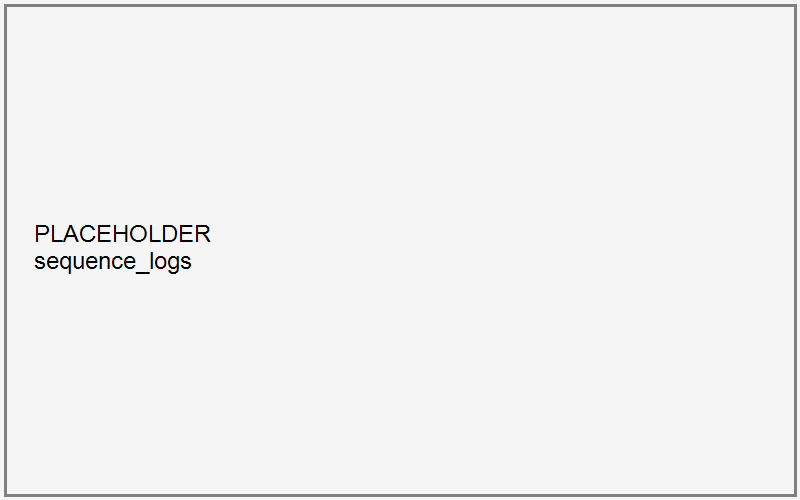
\includegraphics[width=14cm]{diagrammes/sequence_logs.png}
    \caption{Diagramme de séquence — Consultation des journaux en temps réel}
    \label{fig:seq-logs}
\end{figure}

\subsection{Difficultés rencontrées et solutions apportées}

\begin{itemize}
    \item \textbf{Récupération de journaux vide sur les pods Knative} : un pod géré par Knative Serving contient systématiquement deux conteneurs (le conteneur applicatif \texttt{user-container} et le conteneur \textit{sidecar} \texttt{queue-proxy}) ; l'appel initial de récupération des journaux ne précisait pas le conteneur cible et retournait donc un résultat ambigu ou vide. \textit{Solution} : ciblage explicite du conteneur \texttt{user-container} dans les appels Fabric8 de récupération de journaux.
    \item \textbf{Métriques du backend jamais collectées par Prometheus} : les ressources \texttt{ServiceMonitor} et les règles d'alerte du backend portaient une étiquette (\texttt{release: prometheus}) ne correspondant pas au sélecteur réellement configuré sur l'opérateur Prometheus du cluster (\texttt{release: monitoring-stack}), de sorte que les métriques applicatives du backend n'étaient, en pratique, jamais scrutées. Cette anomalie a été identifiée lors de l'audit de la plateforme ; sa correction n'était \textbf{pas encore confirmée en production} au moment de la rédaction de ce mémoire et est reprise comme limite au chapitre de validation.
    \item \textbf{Métrique de requêtes par seconde erronée} : le tableau de bord de supervision du cluster affichait initialement une valeur nulle pour le débit de requêtes, en raison de l'utilisation d'un nom de métrique Prometheus incorrect (\texttt{activator\_request\_count} au lieu de \texttt{revision\_request\_count}). \textit{Solution} : correction du nom de métrique interrogé.
\end{itemize}

\subsection{Résultat obtenu}

Au terme de cette release, la plateforme permet aux clients de suivre en temps réel l'activité de leurs applications, et à l'équipe d'exploitation de superviser l'état global du cluster et d'être alertée automatiquement en cas de dysfonctionnement récurrent d'une application, avec une anomalie de collecte de métriques backend identifiée et non encore définitivement corrigée.

\subsection{Conclusion du Sprint}

Ce sprint clôt la Release 2. La plateforme dispose désormais de l'ensemble des capacités de gestion applicative (applications, Kafka, Eventing) et de supervision nécessaires à son exploitation. La Release 3, objet du chapitre suivant, se concentre sur la livraison de l'interface graphique exposant l'ensemble de ces fonctionnalités aux utilisateurs finaux, ainsi que sur l'industrialisation du pipeline CI/CD.

\section{Conclusion}

La Release 2 a consolidé la couche de services de la plateforme en exposant, de manière sécurisée et isolée par tenant, la gestion de Kafka et de l'Eventing, et en dotant le système de capacités d'observabilité indispensables à son exploitation réelle. Comme pour les releases précédentes, plusieurs anomalies concrètes ont été identifiées et corrigées, à l'exception notable de la collecte de métriques du backend, dont la correction reste à confirmer — un point traité en toute transparence dans le chapitre de validation.
